\section{Redegørsel for Mindste Kvadraters Metode}\label{sec:redegorsel}
Antag at du har en række data. Disse data beskriver en sammenhæng mellem tid og distance for en bil. Bilen kører med en konstant hastighed. Du har nu brug for at finde ud af hvor langt bilen har kørt efter 10 sekunder. Dette ingår dog ikke i datasættet. For at finde denne information kunne man fx. opstille en funktion der beskriver denne sammenhæng. For at beskrive denne sammenhæng, kunne Mindste Kvadraters Metode anvendes. Mindste Kvadraters Metode anvendes ofte til at beskrive en ret linje. (\begin{math}y = ax + b\end{math}) En ret linje kan beskrives på mange måder. Dog vil der kun være en linje der beskriver datasætte bedst. For at finde frem til det krever det, at der fordybes i funktioner af to variable, samt hvordan de afledes.

% Redegør for matematikken bag Mindste Kvadraters Metode (Få sammen sat afsnitet funktioner med to variable og Mindste Kvadraters Metode på en god måde)

\subsection{Funktioner med to variable?}\label{sec:FunktionerMedToVariable}
Du har måske stiftet bekendtskab med funktioner af én variabel. Disse funktioner skrives ofte som $f(x) = x^2$, hvor man indsætter en værdi for $x$ og beregner den tilsvarende værdi af $f(x)$. Her giver man altså en værdi og får en værdi tilbage. Men hvad nu hvis du skal beskrive en sammmenhæng, der er afhængig af to variabler? Her kommer funktioner med to variabler ind i billedet. Når der arbejdes med funktioner af en variabel vil den grafiske afblidning forgå i et koordinatsystem med en x-akse og en y-akse. Altså et todimensionelt koordinatsystem. For at kunne afbillede funktioner af to variable, arbejdes der ikke længere i et koordinatsystem, med todimensioner, men i et tredimensionelt koordinatsystem. Her er der en x-akse, en y-akse og en z-akse. Den nye akse (z-aksen) står vinkelret på de to andre akser (\cite[246-248]{funktionrAfToVariable}). For at bedre forstå, hvordan det tredimensionelle koordinatsystem hænger sammen, kan man tænke på det som en kasse, hvor  $x-aksen$ er længden, $y$-aksen er bredden, og $z-aksen$ er højden. Når der arbejdes med funktioner af to variable, vil den typiske notation se således ud: $f(x,y)$. Her er både $x$ og $y$ variable. Disse to variable kan bruges til at beskrive et punkt i det tredimensionelle koordinatsystem. Dette skyldes, at $z = f(x,y)$. Et eksempel kunne være et vejrkort, hvor temperaturen ($z$) afhænger af geografiske koordinater ($x, y$). Her angiver $x$ og $y$ en lokation, og $z$ angiver temperaturen ved dette punkt. På den måde afhænger temperaturen af to variable, nemlig det geografiske punkt, som beskrives ved $(x, y)$. \\
I forbindelse med Mindste Kvadraters Metode bruges funktioner af to variable til at beskrive summen af kvadraternes areal mellem punkt og en linje. I denne sammenhæng opstilles funktionen $f(a, b)$, hvor $a$ og $b$ er de parametre, der bestemmer linjens hældning og skæring. Denne funktion kan opfattes som en flade i et tredimensionelt koordinatsystem. 
For at finde den linje, der bedst passer til datasættet, skal værdierne af $a$ og $b$ findes. Dette kræver, at der arbejdes med metoder til at finde minimumspunkter i funktioner af to variable. Grunden til hvorfor minimumspunktet skal findes forklares i afsnit \ref{sec:bedsteFunktion}. Hvordan minimumspunktet findes forklares dog i næste afsnit.
% Hvad mangler der at blive redegjort for i dette afsnit? Grafisk afblidning af funktion. Saddelpunkt?)


\subsubsection{Partielt differentiation}\label{sec:PartieltDifferentiation}
For at finde hældningen af tangenten til en funktion af to variable, skal man gå igennem en lidt længere proces end ved funktioner af en variabel. For at finde hældningen af tangenten til funktionen af en variabel, diffrencere man med hensyn til $x$. Et eksempel kunne være $f(x) = x^2$ her er $f'(x) = 2x$. Dette skyldes følgende regneregl: $a \cdot x^n$ bliver til $a \cdot n \cdot x^{n-1}$. \\ Ved funktioner af to variable krærver dette at man benytte sig af en metode kaldt: \textit{Partial differentiation}. Ved partial differentiation, tages der fat i en variabel ad gangen. Partial betyder delvis. Grunden til at dette ord anvendes er da man diffrencere mht. $x$ og $y$ i hver deres led (\cite[4]{Larsen2016}). Her undersøges, hvordan funktionen ændrer sig med hensyn til en variabel, mens den anden betragtes som konstant. Opgaven er nu at finde den partial aflededet funktionen. For at finde den partielle afledede for funktionen $f(x,y)$ startes der med at sætte en af variablerne til en konstant. I dette tilfælde sættes $y$ til en konstant. Når der diffrenceres med en funktion af en variabel, agives dette sådan: \begin{equation}\frac{d f(x)}{d x}\end{equation} Sådan er det dog ikke ved partial differentiation. Her angives det sådan: \begin{equation}\frac{\partial f(x,y)}{\partial x}\end{equation} 
Det bløde $d$ ($partial$) angiver at der differentieres partielt. For at illustrere dette kan funktionen $f(x,y) = x^2 + 3y^2$ tages som eksempel. Målet er at finde de partielle afledede af $f(x,y)$. Først diffrenceres der med hensyn til $x$, mens $y$ dermed betragtes som en konstant. Regnereglerne forskriver at en konstant bliver til nul når den diffrenceres. Dernest anvendes regnereglen, der forskriver at \begin{math}a \cdot x^n\end{math} bliver til \begin{math}a \cdot n \cdot x^{n-1}\end{math} \cite[14]{Pihl2019}. Dermed må den partial aflededet mht. x være: 
\begin{equation}\frac{\partial f(x,y)}{\partial x} = 2x\end{equation}
På samme måde findes den partielle afledede med hensyn til $y$ ved at betragte $x$ som konstant. Dette giver:
\begin{equation}\frac{\partial f(x,y)}{\partial y} = 6y\end{equation}
Ved Mindste Kvadraters Metode anvendes denne teknik til at finde ekstremumspunkter for funktioner af to variable. Ekstremumspunkterne repræsenterer de værdier for parametrene $a$ og $b$, der minimerer summen af kvadrerede afvigelser mellem datapunkterne og modellen. Dette uddybes i det følgende afsnit.
\newpage
\subsection{Sådan finder du frem til den bedste funktion}\label{sec:bedsteFunktion}
I de foregående afsnit er der blevet redegjort for funktioner af to variable og, hvordan de differentieres. Der er også blevet forklaret, hvorfor disse metoder er relevante, og hvordan de kan bruges i forbindelse med Mindste Kvadraters Metode. For at finde den bedste funktion skal der først udvikles en metode til at beskrive, hvor godt en funktion passer til et datasættet. Den nemmeste måde at beskrive hvor godt en linje passer på et datasæt vil nok være at beskrive afstanden fra punkt til linje. Dette kan gøres på flere måder. Afstanden kunne være den vinkelrette afstand fra linjen ned til punktet. dette er dog ret svært at regne med. I stedet for det kan den lodrette afstand fra punkt til linje findes. Dette gøres ved at finde forskellen i y-værdierne.
\begin{wrapfigure}{r}{0.5\textwidth}
    \centering
    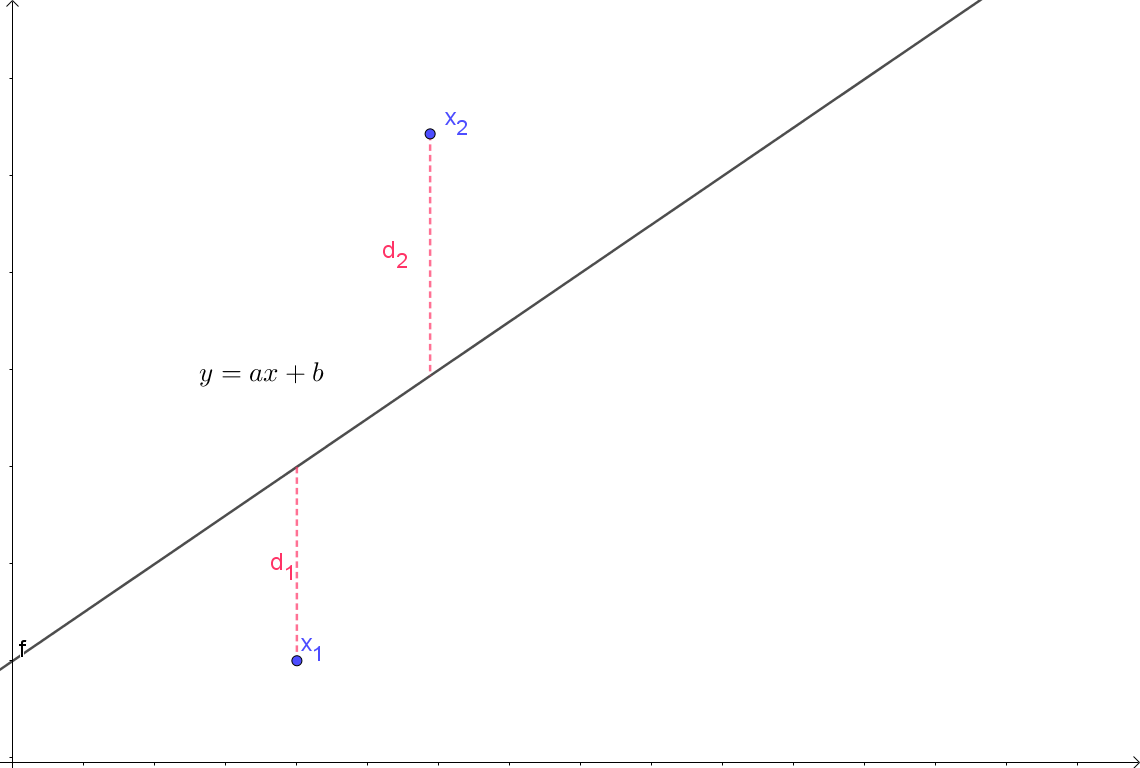
\includegraphics[width=0.5\textwidth]{figures/afstand.png}
    \caption{Afstand fra punkt til linje}
    \label{fig:afstandFraLinjeTilPunkt}
\end{wrapfigure}   
Dette skaber dog en udfordring som man skal være opmærksom på. Nemlig at der kan være punkter over og under linjen. En distance kan altså derfor både være positiv og negativ. For at undgå at dette bliver et problem opløftes afstanden i anden. (\cite[2]{ForberedelsessetMaj2013}). Se figur \ref{fig:afstandFraLinjeTilPunkt} for grafisk ilustration \\ Da der nu er styr på hvordan afstanden fra punkt til linje findes. Skal der nu findes en metode hvorpå det er muligt at beskrive afstanden ift linjen. Hvis der startes med at tage udgangspunkt i et punkt. Punktet kunne hede hvad somhelst. Linjen hedder dog altid: $y = a \cdot x + b$. Så må afstanden i y-værdien kunne beskrives som:  
\begin{equation}\label{eq:distance}
    d_n = a \cdot x_n + b - y_n
\end{equation} grunden til at $y_n$ fratrækkes, er at y-værdien for linjen ved $x_n$ ville være $y = a \cdot x + b$. Isoleret set så er afstanden y-værdien for funktionen minus y-værdien for punktet. På den måde kan afstanden altså bestemmes. Afstanden har på den måde nu dannet en ligning med to ubekendt. Til sammen beskriver de arealet af en kvadrat. Grunden til at de beskriver arealet af en kvadrat er da afstanden som nævnt før opløftes i anden. Det må derfor være det samme som at regne arealet af en kvadrat (\cite{Bentzen2014}). Nu begynder navnte Mindste Kvadraters Metode lige så stille at give mening. Da målet er at finde den linje hvor Kvadraternes areal er mindst. For at regne distance fra alle punkter til linjne anvendes den formlen som blev introduceret før (Formel: \ref{eq:distance}). Deres fælles areal kan derfor beskrives som følgende:
\begin{equation}\label{eq:formularForDistanceForAllDataPoints}A = \sum_{n=1}^n (a \cdot x_n + b - y_n)^2\end{equation}
Resultat af denne udregning kunne omskrives til en funktion af to variable, hvor $a$ og $b$ er de ubekendte. Der hvor arealerne er mindst må de to ubekendte danne den best mulige linje. Dette ville kunne ses som et ekstrema, på funktionen af variablerne $a$ og $b$. Dette ekstrema findes ved at lave partial diffrencering (Se afsnit \ref{sec:PartieltDifferentiation}) af funktionen med hensyn til $a$ og $b$ og til sidst sætte differentialkvotienterne til 0. Dette skyldes at når hældningen af tangenten er nul så vil der være enten et toppunkt eller minimumspunkt. I tildfældet her vil der kun være et minimumspunkt. Da slut funktionen danner en parabel ligende figur. Der vil nu være dannet to ligninger med med to ubekendte, vil være hhv $a$ og $b$ Disse to ligninger kan løses og dermed findes den bedste linje. (\cite{webmatematikMindsteKvadratersMetode})

\section{Praktisk anvendelse af Mindste Kvadraters Metode}\label{sec:udregning}
Med baggrund i afsnit \ref{sec:redegorsel} om redegørsel for Mindste Kvadraters Metode kan metoden nu anvendes på datasættet om bilen, der kører med konstant hastighed. Datasættet viser sammenhængen mellem tid og den tilbagelagte distance for bilen:
\begin{table}[h!]
    \centering
    \begin{tabular}{|c|c|} \hline
        $Tid [s]$ & $Distance [m]$ \\ \hline
        $1$ & $6$ \\ 
        $5$ & $6$ \\
        $6$ & $12$ \\
        $10$ & $10$ \\ \hline
    \end{tabular}
    \caption{Sammenhæng mellem tid og distance.}
\end{table}\\
For at finde frem til den funktion, der bedst beskriver datasættet, opstilles først den ligning som blev forklaret for oven (Formel: \ref{eq:formularForDistanceForAllDataPoints}), der beskriver afstanden mellem punkterne og linjen:
\begin{equation*}
    A = (a \cdot 1 + b - 6)^2 + (a \cdot 5 + b - 6)^2 + (a \cdot 6 + b - 12)^2 + (a \cdot 10 + b - 10)^2
\end{equation*}
Dette udtryk skal udvides, så alle ledene med $a$, $b$ og $ab$ er samlet et sted.Første skridt er at omskrive hvert kvadrat så det kommer på denne form: 
\begin{equation*}
    (a \cdot x_n + b - y_n)^2 = (a \cdot x_n + b - y_n) \cdot (a \cdot x_n + b - y_n)
\end{equation*}
Dette gør det muligt at udvide udtrykkene ved at gange parenteserne ud. Alle led tages nu hvert for sig og udvides:\\
\textbf{Punktet} $\mathbf{(1,6)}$ \textbf{udvidet:}
\begin{equation*}
    (a \cdot 1 + b - 6) \cdot (a \cdot 1 + b - 6) = a^2 + b^2 + 2ab - 12a - 12b + 36
\end{equation*}
\textbf{Punktet} $\mathbf{(5,6)}$ \textbf{udvidet:}
\begin{equation*}
    (a \cdot 5 + b - 6) \cdot (a \cdot 5 + b - 6) = b^2 + 10ab -12b + 25a^2 - 60a + 36
\end{equation*}
\textbf{Punktet}   $\mathbf{(6,12)}$ \textbf{udvidet:}
\begin{equation*}
    (a \cdot 6 + b - 12) \cdot (a \cdot 6 + b - 12) = b^2 + 12ab - 24b + 36a^2 - 144a + 144
\end{equation*}
\textbf{Punktet}   $\mathbf{(10,10)}$ \textbf{udvidet:}
\begin{equation*}
    (a \cdot 10 + b - 10) \cdot (a \cdot 10 + b - 10) = b^2 + 20ab - 20b + 100a^2 - 200a + 100
\end{equation*}
Alle led samles nu til et samlet udtryk. 
\begin{equation*}
    \begin{split}
    A = a^2 + b^2 + 2ab - 12a - 12b + 36 + b^2 + 10ab -12b + 25a^2 - 60a + 36 + \\ b^2 + 12ab - 24b + 36a^2 - 144a + 144 + b^2 + 20ab - 20b + 100a^2 - 200a + 100
\end{split}
\end{equation*}
Dette udvidet udtrykket kan nu reduceres til:
\begin{equation*}
    A = 44ab - 68b + 4b^2 - 416a + 162a^2 + 316
\end{equation*}
Dette omskrives til en funktion af to variabele, hvor $a$ og $b$ er de ubekendte. 
\begin{equation*}
   f(a,b) = 44ab - 68b + 4b^2 - 416a + 162a^2 + 316 
\end{equation*}
\begin{figure}[h!]
    \centering
    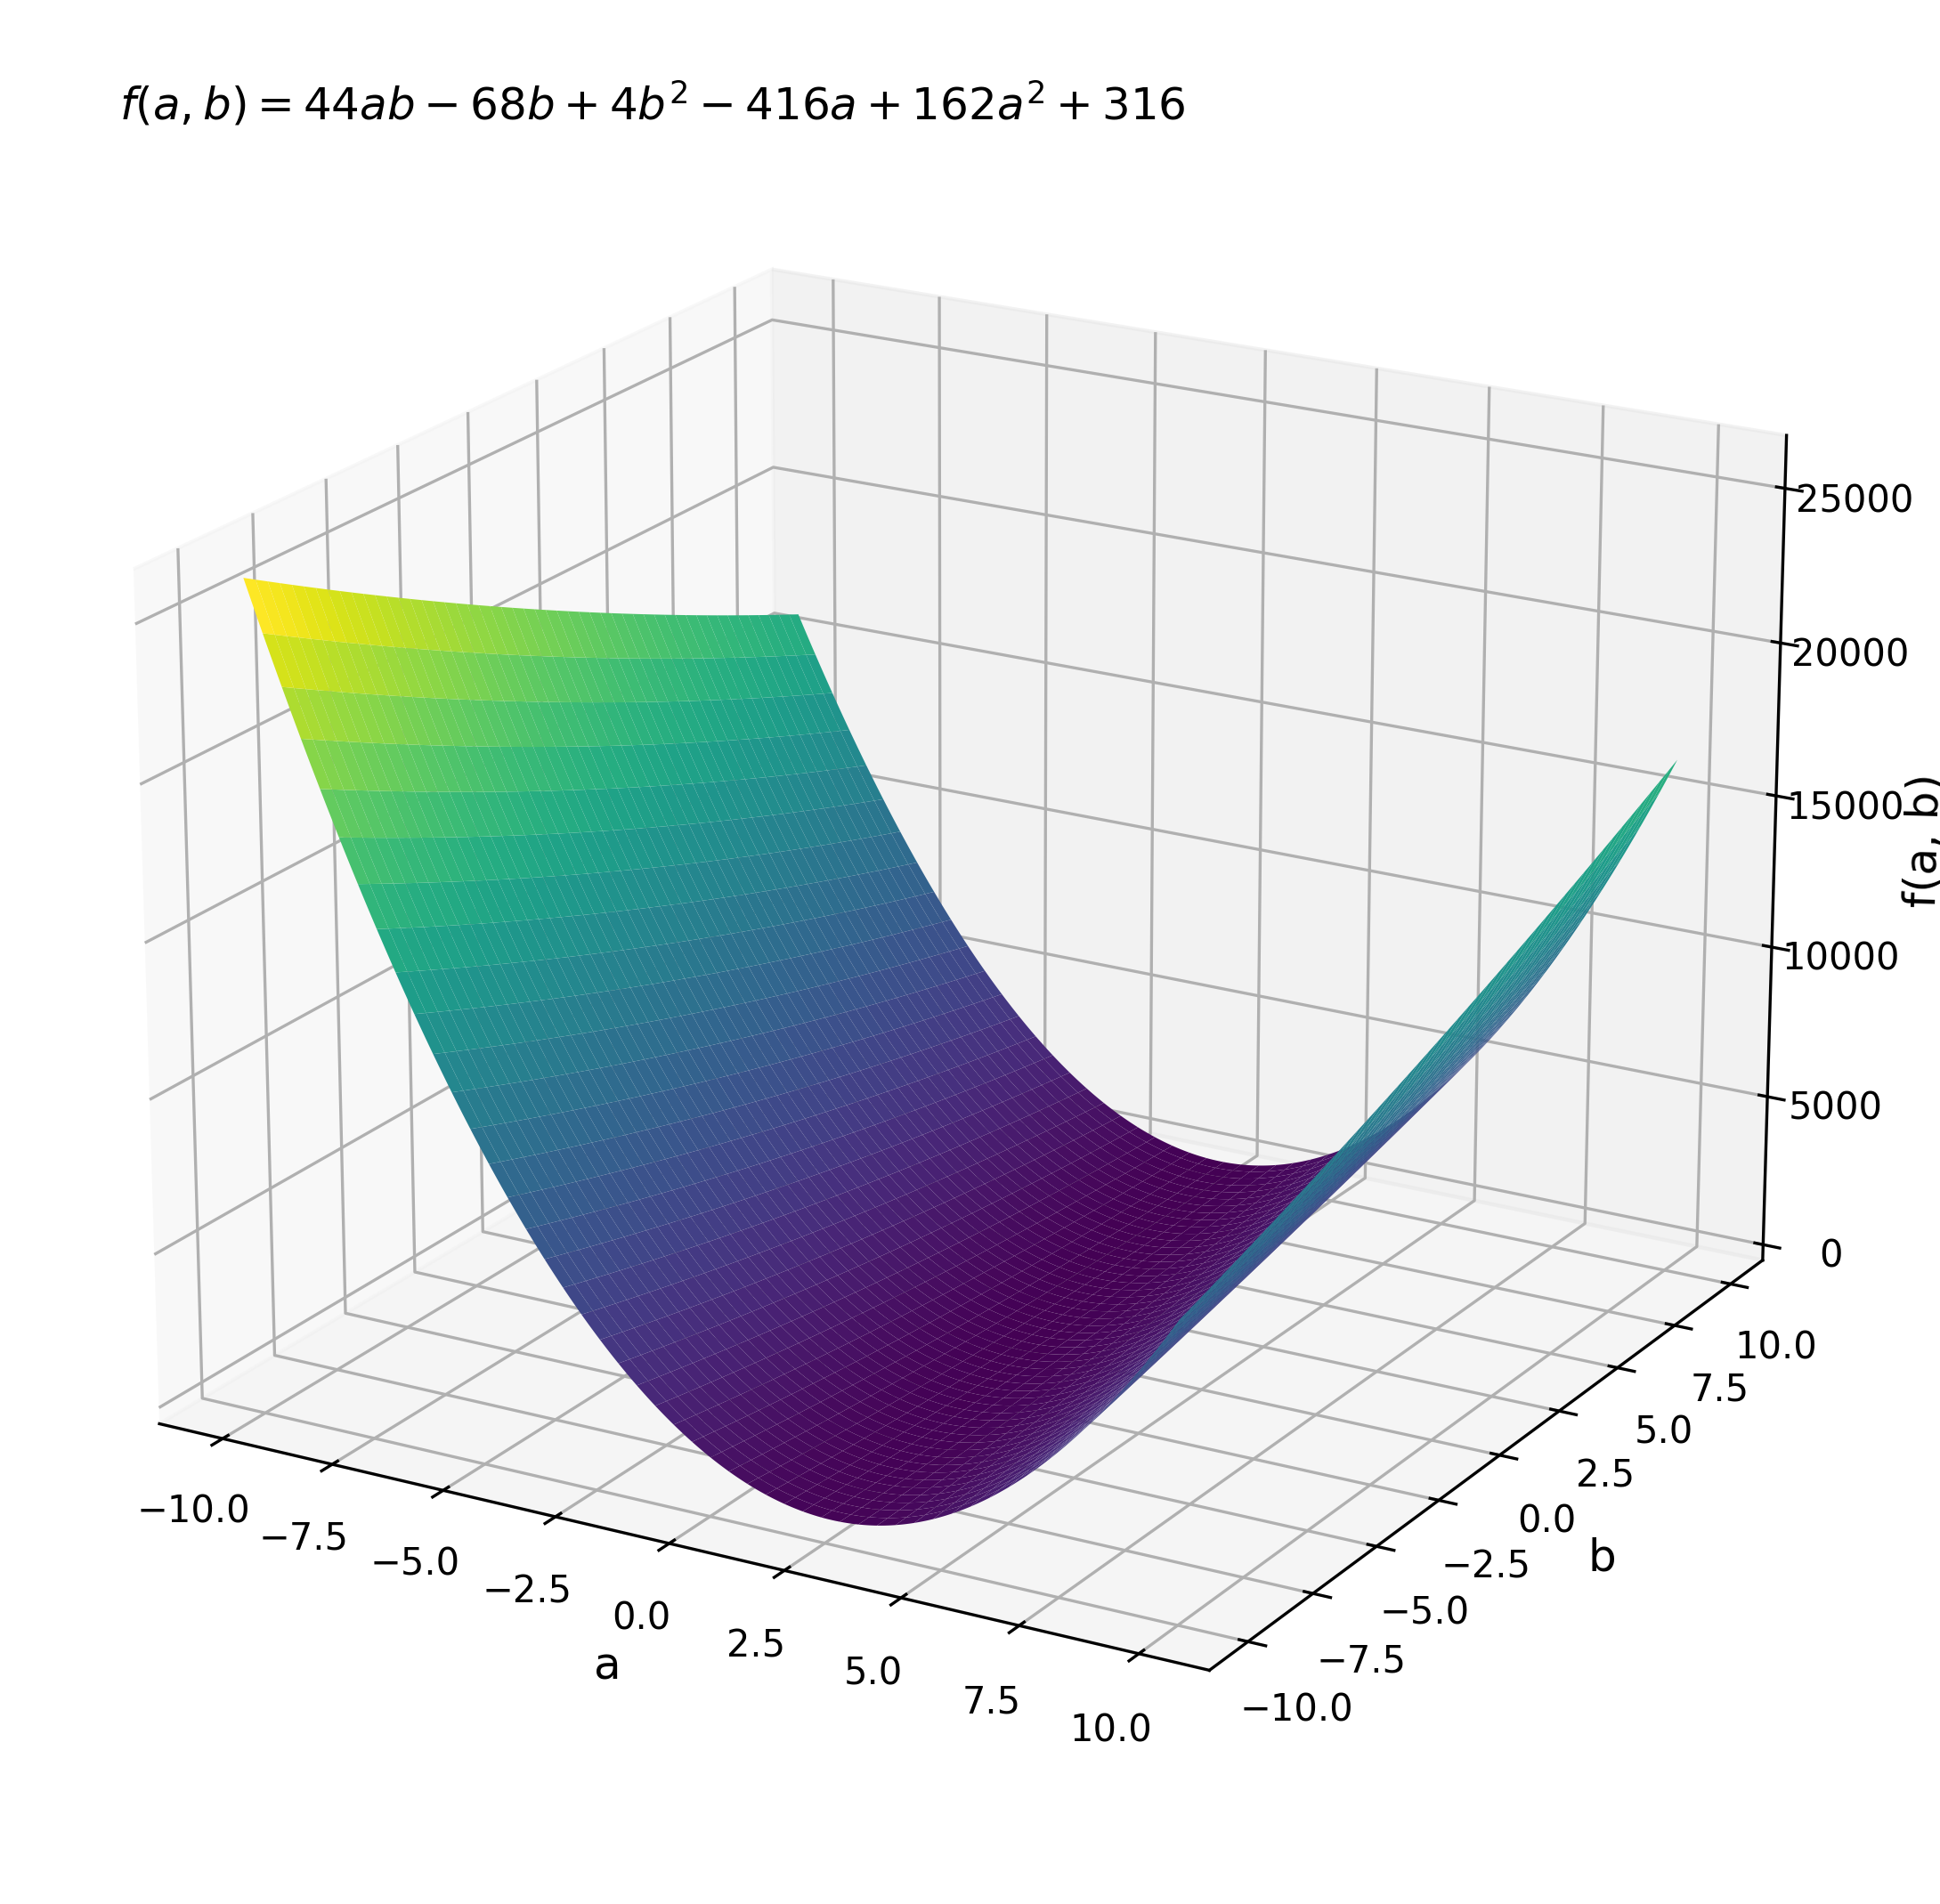
\includegraphics[width=0.5\textwidth]{figures/3dGraf.png}
    \caption{Grafisk afblidning af funktionen $f(a,b)$}
    \label{fig:grafiskAfbildningAfFunktionAfToVariable}
\end{figure}  
For at finde den funktion der passer bedst til datasættet, skal der findes det sted hvor funktionen $f(a,b)$ har et minimumspunkt (Se evt figur \ref{fig:grafiskAfbildningAfFunktionAfToVariable}) Dette gøres ved at tage partielt afledede af funktionen $f(a,b)$ med hensyn til $a$ og $b$. De differentialkvotienter der kommer ud af dette sættes til 0. 
\begin{equation*}
    \frac{\partial f(a,b)}{\partial a} = 44b + 324a - 416
\end{equation*}
\begin{equation*}
    \frac{\partial f(a,b)}{\partial b} = 8b + 44a - 68
\end{equation*}
Disse to difransialkvotienter sættes nu til 0. Dette giver følgende ligningsystem:
\begin{equation*}
    44b + 324a - 416 = 0
\end{equation*}
\begin{equation*}
    8b + 44a - 68 = 0
\end{equation*}
Dette ligningsystem kan nu løses med hensyn til $a$ og $b$. Dette giver følgende resultat: % Måske vise hvordan to ligninger løses
\begin{equation*}
    a = 0,5122 
\end{equation*}
\begin{equation*}
    b = 5,68293
\end{equation*}
Resultatet af beregningerne af dette datasæt viser at denne metode godt, kan anvendes til at finde en linje der passer bedst til et datasæt. Det kan være svært at konkludere præcist hvor god den er, men resultatet er sat op mod GeoGebra og her stemmer resultaterne overens, helt ned til 5 decimal.
% Synes stadig ikke helt at jeg er i mål med denne del. 

\section{Programmering og Matematik i samspil}
Matematik og programmering hænger på mange måder naturligt godt sammen. Matematik bruges til at beskrive og forklare komplekse problemstillinger, mens programmering gør det muligt at omsætte disse problemstillinger til konkrete løsninger. Med programmering følger også en række praktiske fordele, som kan gøre selv de sværeste håndberegninger på sekunder. Dette gælder især, når man arbejder med store datasæt. Programmering giver os værktøjerne til at bearbejde data hurtigt og præcist, hvilket er noget, mennesker aldrig ville kunne gøre manuelt lige så hurtigt. (\cite{codeWithC}) Forestil dig for eksempel, at du har ti tusinde datapunkter fra en virksomheds salgsdata. At finde et mønster manuelt ville være en næsten umulig opgave. Her kommer computeren og programmeringen ind i billedet. Ved hjælp af simple algoritmer og lidt programmeringserfaring kan man omsætte dataene til resultater på få sekunder. Det samme gælder, når der arbejdes med Mindste Kvadraters Metode. Hvor det manuelt ville kræve mange trin og lang tid at finde den bedst passende linje, kan en computer beregne dette på ingen tid. Se bare hvor mange skridt der er blevet taget i afsnit \ref{sec:udregning} for at finde den bedst mulige linje, tænk på hvor lang tid det ville tage hvis der var mere end fire punkter. Programmering er ikke bare hurtigere. Det åbner også op for at eksperimentere og tilpasse løsninger. Har man for eksempel data, hvor nogle observationer afviger markant fra de andre resultater, kan man justere modellen eller filtrere data for at få en bedre beskrivelse. Med Mindste Kvadraters Metode kan det også hurtigt testes, hvordan små ændringer i datasættet påvirker slut resultatet. Denne fleksibilitet er især hvis det data der kommer ud af et forsøg ikke opføre sig som forventet. Muligheden for at ændre beregninger undervejs, er dog ikke den eneste fordel, som kommer da programmering anvendes. En anden fordel ved at kombinere matematik og programmering er muligheden for at visualisere. Når en model er blevet beregnet, kan man hurtigt lave grafer, der viser, hvordan modellen passer til det konkrete datasæt. For eksempel kan man plotte en lineær regression sammen med de oprindelige datapunkter for at få et visuelt overblik over, hvordan sammenhængen ser ud. Det gør resultaterne nemmere at forstå og formidle. Det er netop i kombinationen af matematik og programmering, at den virkelige styrke ligger. Matematikken giver præcision og struktur, mens programmeringen giver hastighed, fleksibilitet og mulighed for at arbejde med data i stor skala. Dette gør ikke bare processen hurtigere, men det gør det også muligt at håndtere komplekse problemstillinger, som tidligere ville have været uden for rækkevidde. Når man arbejder med metoder som Mindste Kvadraters Metode, bliver denne kombination særlig tydelig. Det er her, de abstrakte modeller møder den praktiske virkelighed, og resultaterne bliver noget, man faktisk kan bruge (\cite{geeksforgeeks}). \\

\section{Implementering af Mindste Kvadraters Metode}
Som tidligere nævnt er en af styrkerne ved at anvende programmering dens evne til at automatisere og effektivisere beregninger. Dette er en stærkt fordel, når der arbejdes med Mindste Kvadraters Metode. Hvor det manuelt ville tage mange trin at finde den bedst passende linje, gør programmering det muligt at omsætte de matematiske beregninger til kode, der hurtigt og præcist kan håndtere selv store datasæt. Dette åbner op for en række anvendelser, lige fra praktisk dataanalyse til visualisering og optimering. I dette afsnit vil der blive fokuseret på, hvordan Mindste Kvadraters metode kan implementeres i programmering (\cite{geeksforgeeks2}). Ved at anvende en struktureret tilgang kan de matematiske formler opdeles i klare og logiske trin, som nemt kan oversættes til kode. Pseudokode fungerer som et effektivt værktøj til at beskrive denne proces på en enkel og overskuelig måde.

\subsection{Pseudokode for Mindste Kvadraters Metode}
For at implementere Mindste Kvadraters Metode er det vigtigt at det hele tiden anvendes en struktureret tilgang, hvor de nødvendige matematiske operationer udføres trin for trin. Følgende er en pseudokode, der beskriver, hvordan Mindste Kvadraters Metode kan implementeres i programmering:
\begin{algorithmic}[1] 
        \REQUIRE Datasæt \((x_1, y_1), (x_2, y_2), \dots, (x_n, y_n)\)
        \STATE Start
        \STATE \textbf{Opret:}
        \STATE \hspace{0.5cm} sum\_a2 = 0 
        \STATE \hspace{0.5cm} sum\_b2 = 0  
        \STATE \hspace{0.5cm} sum\_ab = 0  
        \STATE \hspace{0.5cm} sum\_a = 0   
        \STATE \hspace{0.5cm} sum\_b = 0  
        \STATE \hspace{0.5cm} konstant\_sum = 0
        
        \STATE \textbf{For hvert datapunkt $\mathbf{(x_i, y_i)}$ i datasættet:}
        \STATE Indset i formlen $(a \cdot x_i + b - y_i)^2$
        \STATE \hspace{0.5cm} Udvid \((a \cdot x_i + b - y_i)^2\)
        \STATE \hspace{0.5cm} Beregn bidragene til \(a^2\), \(b^2\), \(ab\), og konstanter
        \STATE \hspace{0.5cm} Tilføj disse værdier i sum\_a2, sum\_b2, sum\_ab, sum\_a, sum\_b, og konstant\_sum
        
        \STATE \textbf{Kombiner alle bidrag i den samlede funktion $\mathbf{f(a,b) }$:}
        \STATE \hspace{0.5cm} $f(a, b) = sum a2 + sum b2 + sum ab + sum a + sum b + konstant sum$        
        \STATE Find den partielt aflededet for funktionen $f(a, b)$:
        \STATE \hspace{0.5cm} $\frac{\partial f}{\partial a}$
        \STATE \hspace{0.5cm} $\frac{\partial f}{\partial b}$
        
        \STATE Find frem til $a og b$ ved at sætte differentialkvotienterne til 0:
        \STATE \hspace{0.5cm} \(\frac{\partial f}{\partial a} = 0\)
        \STATE \hspace{0.5cm} \(\frac{\partial f}{\partial b} = 0\)
        
        \RETURN \(a, b\)
\end{algorithmic}
Denne pseudokode illustrerer, hvordan Mindste Kvadraters Metode kan implementeres trin for trin i et programmerings øjemed. De matematiske beregninger, som blev beskrevet tidligere, bliver til en proces, der hurtigt og præcist kan håndtere data (\cite{codesansar}). At anvende Pseudokode virker i sig selv, måske lidt irelevandt. Det kan dog være med til at give et bedre overbil over hvordan Mindste Kvadraters Metode kan implementeres i programmering, og hvordan matematik og programmering kan arbejde sammen om at løse komplekse problemstillinger.

\subsection{Program Design}
Afsnittet om pseudokode har givet et godt overblik over, hvordan Mindste Kvadraters Metode kan implementeres i programmering. Der er dog flere overvejelser, der skal gøres. At skrive et program, er ikke bare at skrive et program. Det kræver en grundig planlægning og overvejelse af, hvordan programmet skal designes, hvilke sprog og biblioteker der skal anvendes, og hvordan det hele skal hænge sammen. Det bedste sted at starte ved et hvert program er: hvad er formålet med programmet? Formålet med programmet her, er at implementere Mindste Kvadraters Metode for at fidne den bedst passende linje til et givet datasæt. Designet af programmet er baseret på nøje overvejelser om skalerbarhed, fleksibilitet, og muligheden for nemt ændre i forskellige dele af programmet. En vigtig overvejelse i designet har været, hvilket paradigme der skulle anvendes. Skulle programmet være objektorienteret, funktionelt, eller noget helt tredje? Alt sammen kommer med deres fordele og ulemper. Mere om dette i afsnittet om Kodningsmetoder (Afsnit: \ref{sec:Kodningsmetoder}). Grunden til at valget af paradigme endte på funktionelt programmering, er at det giver en række klare fordele når det kommer til modularitet (\cite{gupta}). En af de helt store årsager til at funktionelt programmering er valgt over objektorienteret er at funktionel programmering i højere grad fremmer "immutability" (Datastruktur eller et objekt ikke kan ændres efter, det er blevet oprettet) og modularitet, hvilket gør at det lettere at tilføje eller ændre funktionalitet løbende uden at påvirke andre dele af programmet. Dette kan især være vigtigt i tilfælde, hvor man ønsker at håndtere data, der ændres dynamisk, eller hvor man skal beregne nye resultater baseret på forskellige datasæt. Funktionel programmering tilbyder en række værktøjer og principper, såsom højere-ordens funktioner og renhed (pure functions), der gør det lettere at arbejde med komplekse matematiske operationer som Mindste Kvadraters Metode (\cite{funktionelProgrammering}). Hvis man derimod skulle implementere Mindste Kvadraters Metode i et objektorienteret paradigme, ville man typisk skulle bruge flere ressourcer på at administrere tilstande og objekter. For eksempel kan det kræve flere klasser og metoder til at definere og opdatere de forskellige parametre, som  $a$ og $b$, samt opbevare datasættet. \\  
Når det kommer til sprogvalg, så faldt beslutningen på Python. Dette valgt blev truffet på baggrund af sprogets forcer. Python er et af de mest populære programmeringssprog i verden, hvilket betyder, at der er masser af dokumentation og biblioteker til rådighed. Dette er dog ikke det eneste der gør Python til et godt valg. Python er desuden kendt for sin enkelhed og læsbarhed, hvilket gør det nemt at skrive og vedligeholde kode. Dette er en stor fordel, især i projekter, hvor klarhed og hurtig implementering er vigtig. \\\\
En anden væsentlig styrke ved Python er dets evne til at håndtere store datasæt effektivt, hvilket er centralt i dette projekt. Med biblioteker som NumPy og SciPy kan komplekse matematiske beregninger, som dem der kræves til Mindste Kvadraters Metode, udføres hurtigt og præcist. Selv om andre sprog som C og Java også kunne løse opgaven, blev Python valgt, fordi det tillader hurtigere udvikling og lettere forståelse af koden. Disse egenskaber gør Python til et oplagt valg til dette projekt (\cite{simplilearn}). \\\\
I programdesign spiller ikke kun valget af sprog og paradigme en rolle, men også hvordan koden struktureres og dokumenteres. Et godt dokumenteret program gør det muligt for andre (eller en selv) at forstå og ændre koden i fremtiden. Kommentarer og klare funktionsbeskrivelser er en stor del af designet og sikrer, at koden er så selvforklarende som muligt. Samtidig understøtter Python brugen af docstrings, som giver en struktureret måde at dokumentere hver funktion og dens formål på.
Alt i alt er programmets design med til at sikre, at det er nemt at vedligeholde, forstå og udvide. Ved at bygge programmet med baggrund i de før nævnte principper sikres det, at det ikke kun opfylder dets nuværende formål: at implementere Mindste Kvadraters Metode. Men også forbliver robust og fleksibelt nok til at håndtere fremtidige behov og anvendelser. Dette gør programmet til en bæredygtig løsning.

\subsection{Program redegørsel}
% Redegør for programmet og dets funktioner (Husk at inkludere kodeeksempler)

\section{Fordele og Begrænsninger}\label{sec:fordeleOgBegrensninger}
%Her analyseres metoden på et bredere niveau ved at vurdere dens styrker og svagheder i en programmeringssammenhæng.

\section{Diskussion af Kodningsmetoder}\label{sec:Kodningsmetoder}
% While loops, for loops, rekursive funktioner, ect.

\section{Konklusion}

\section{Perspektivering}
